% Created by tikzDevice version 0.7.0 on 2015-09-03 08:33:27
% !TEX encoding = UTF-8 Unicode
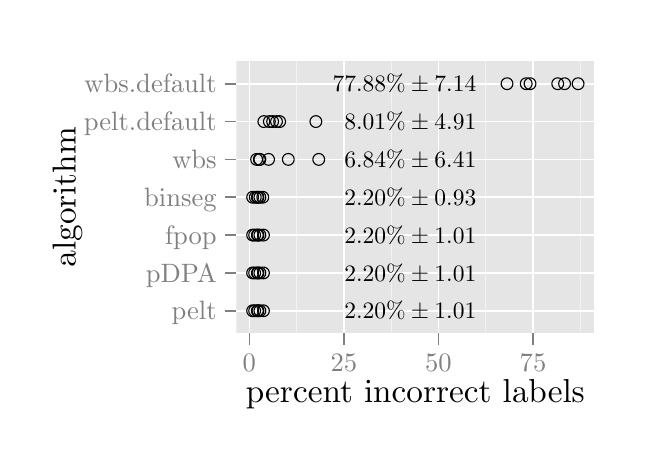
\begin{tikzpicture}[x=1pt,y=1pt]
\definecolor[named]{fillColor}{rgb}{1.00,1.00,1.00}
\path[use as bounding box,fill=fillColor,fill opacity=0.00] (0,0) rectangle (216.81,144.54);
\begin{scope}
\path[clip] (  0.00,  0.00) rectangle (216.81,144.54);
\definecolor[named]{drawColor}{rgb}{1.00,1.00,1.00}
\definecolor[named]{fillColor}{rgb}{1.00,1.00,1.00}

\path[draw=drawColor,line width= 0.6pt,line join=round,line cap=round,fill=fillColor] ( -0.00,  0.00) rectangle (216.81,144.54);
\end{scope}
\begin{scope}
\path[clip] ( 75.41, 34.03) rectangle (204.76,132.50);
\definecolor[named]{fillColor}{rgb}{0.90,0.90,0.90}

\path[fill=fillColor] ( 75.41, 34.03) rectangle (204.76,132.50);
\definecolor[named]{drawColor}{rgb}{0.95,0.95,0.95}

\path[draw=drawColor,line width= 0.3pt,line join=round] ( 97.19, 34.03) --
	( 97.19,132.50);

\path[draw=drawColor,line width= 0.3pt,line join=round] (131.36, 34.03) --
	(131.36,132.50);

\path[draw=drawColor,line width= 0.3pt,line join=round] (165.53, 34.03) --
	(165.53,132.50);

\path[draw=drawColor,line width= 0.3pt,line join=round] (199.70, 34.03) --
	(199.70,132.50);
\definecolor[named]{drawColor}{rgb}{1.00,1.00,1.00}

\path[draw=drawColor,line width= 0.6pt,line join=round] ( 75.41, 42.24) --
	(204.76, 42.24);

\path[draw=drawColor,line width= 0.6pt,line join=round] ( 75.41, 55.91) --
	(204.76, 55.91);

\path[draw=drawColor,line width= 0.6pt,line join=round] ( 75.41, 69.59) --
	(204.76, 69.59);

\path[draw=drawColor,line width= 0.6pt,line join=round] ( 75.41, 83.26) --
	(204.76, 83.26);

\path[draw=drawColor,line width= 0.6pt,line join=round] ( 75.41, 96.94) --
	(204.76, 96.94);

\path[draw=drawColor,line width= 0.6pt,line join=round] ( 75.41,110.61) --
	(204.76,110.61);

\path[draw=drawColor,line width= 0.6pt,line join=round] ( 75.41,124.29) --
	(204.76,124.29);

\path[draw=drawColor,line width= 0.6pt,line join=round] ( 80.10, 34.03) --
	( 80.10,132.50);

\path[draw=drawColor,line width= 0.6pt,line join=round] (114.27, 34.03) --
	(114.27,132.50);

\path[draw=drawColor,line width= 0.6pt,line join=round] (148.44, 34.03) --
	(148.44,132.50);

\path[draw=drawColor,line width= 0.6pt,line join=round] (182.61, 34.03) --
	(182.61,132.50);
\definecolor[named]{drawColor}{rgb}{0.00,0.00,0.00}

\node[text=drawColor,anchor=base east,inner sep=0pt, outer sep=0pt, scale=  0.85] at (162.11, 39.31) {$2.20\% \pm 1.01$};

\node[text=drawColor,anchor=base east,inner sep=0pt, outer sep=0pt, scale=  0.85] at (162.11, 52.99) {$2.20\% \pm 1.01$};

\node[text=drawColor,anchor=base east,inner sep=0pt, outer sep=0pt, scale=  0.85] at (162.11, 66.66) {$2.20\% \pm 1.01$};

\node[text=drawColor,anchor=base east,inner sep=0pt, outer sep=0pt, scale=  0.85] at (162.11, 80.34) {$2.20\% \pm 0.93$};

\node[text=drawColor,anchor=base east,inner sep=0pt, outer sep=0pt, scale=  0.85] at (162.11, 94.01) {$6.84\% \pm 6.41$};

\node[text=drawColor,anchor=base east,inner sep=0pt, outer sep=0pt, scale=  0.85] at (162.11,107.69) {$8.01\% \pm 4.91$};

\node[text=drawColor,anchor=base east,inner sep=0pt, outer sep=0pt, scale=  0.85] at (162.11,121.36) {$77.88\% \pm 7.14$};

\path[draw=drawColor,line width= 0.4pt,line join=round,line cap=round] ( 82.99, 42.24) circle (  2.13);

\path[draw=drawColor,line width= 0.4pt,line join=round,line cap=round] ( 83.91, 42.24) circle (  2.13);

\path[draw=drawColor,line width= 0.4pt,line join=round,line cap=round] ( 81.29, 42.24) circle (  2.13);

\path[draw=drawColor,line width= 0.4pt,line join=round,line cap=round] ( 83.22, 42.24) circle (  2.13);

\path[draw=drawColor,line width= 0.4pt,line join=round,line cap=round] ( 82.02, 42.24) circle (  2.13);

\path[draw=drawColor,line width= 0.4pt,line join=round,line cap=round] ( 85.20, 42.24) circle (  2.13);

\path[draw=drawColor,line width= 0.4pt,line join=round,line cap=round] ( 82.99, 55.91) circle (  2.13);

\path[draw=drawColor,line width= 0.4pt,line join=round,line cap=round] ( 83.91, 55.91) circle (  2.13);

\path[draw=drawColor,line width= 0.4pt,line join=round,line cap=round] ( 81.29, 55.91) circle (  2.13);

\path[draw=drawColor,line width= 0.4pt,line join=round,line cap=round] ( 83.22, 55.91) circle (  2.13);

\path[draw=drawColor,line width= 0.4pt,line join=round,line cap=round] ( 82.02, 55.91) circle (  2.13);

\path[draw=drawColor,line width= 0.4pt,line join=round,line cap=round] ( 85.20, 55.91) circle (  2.13);

\path[draw=drawColor,line width= 0.4pt,line join=round,line cap=round] ( 82.99, 69.59) circle (  2.13);

\path[draw=drawColor,line width= 0.4pt,line join=round,line cap=round] ( 83.91, 69.59) circle (  2.13);

\path[draw=drawColor,line width= 0.4pt,line join=round,line cap=round] ( 81.29, 69.59) circle (  2.13);

\path[draw=drawColor,line width= 0.4pt,line join=round,line cap=round] ( 83.22, 69.59) circle (  2.13);

\path[draw=drawColor,line width= 0.4pt,line join=round,line cap=round] ( 82.02, 69.59) circle (  2.13);

\path[draw=drawColor,line width= 0.4pt,line join=round,line cap=round] ( 85.20, 69.59) circle (  2.13);

\path[draw=drawColor,line width= 0.4pt,line join=round,line cap=round] ( 82.99, 83.26) circle (  2.13);

\path[draw=drawColor,line width= 0.4pt,line join=round,line cap=round] ( 83.91, 83.26) circle (  2.13);

\path[draw=drawColor,line width= 0.4pt,line join=round,line cap=round] ( 81.29, 83.26) circle (  2.13);

\path[draw=drawColor,line width= 0.4pt,line join=round,line cap=round] ( 83.22, 83.26) circle (  2.13);

\path[draw=drawColor,line width= 0.4pt,line join=round,line cap=round] ( 82.25, 83.26) circle (  2.13);

\path[draw=drawColor,line width= 0.4pt,line join=round,line cap=round] ( 84.96, 83.26) circle (  2.13);

\path[draw=drawColor,line width= 0.4pt,line join=round,line cap=round] (105.17, 96.94) circle (  2.13);

\path[draw=drawColor,line width= 0.4pt,line join=round,line cap=round] ( 83.91, 96.94) circle (  2.13);

\path[draw=drawColor,line width= 0.4pt,line join=round,line cap=round] ( 82.72, 96.94) circle (  2.13);

\path[draw=drawColor,line width= 0.4pt,line join=round,line cap=round] ( 83.70, 96.94) circle (  2.13);

\path[draw=drawColor,line width= 0.4pt,line join=round,line cap=round] ( 87.04, 96.94) circle (  2.13);

\path[draw=drawColor,line width= 0.4pt,line join=round,line cap=round] ( 94.18, 96.94) circle (  2.13);

\path[draw=drawColor,line width= 0.4pt,line join=round,line cap=round] ( 87.33,110.61) circle (  2.13);

\path[draw=drawColor,line width= 0.4pt,line join=round,line cap=round] ( 91.05,110.61) circle (  2.13);

\path[draw=drawColor,line width= 0.4pt,line join=round,line cap=round] ( 85.34,110.61) circle (  2.13);

\path[draw=drawColor,line width= 0.4pt,line join=round,line cap=round] ( 88.51,110.61) circle (  2.13);

\path[draw=drawColor,line width= 0.4pt,line join=round,line cap=round] ( 89.91,110.61) circle (  2.13);

\path[draw=drawColor,line width= 0.4pt,line join=round,line cap=round] (104.13,110.61) circle (  2.13);

\path[draw=drawColor,line width= 0.4pt,line join=round,line cap=round] (191.53,124.29) circle (  2.13);

\path[draw=drawColor,line width= 0.4pt,line join=round,line cap=round] (180.15,124.29) circle (  2.13);

\path[draw=drawColor,line width= 0.4pt,line join=round,line cap=round] (198.89,124.29) circle (  2.13);

\path[draw=drawColor,line width= 0.4pt,line join=round,line cap=round] (194.00,124.29) circle (  2.13);

\path[draw=drawColor,line width= 0.4pt,line join=round,line cap=round] (181.53,124.29) circle (  2.13);

\path[draw=drawColor,line width= 0.4pt,line join=round,line cap=round] (173.21,124.29) circle (  2.13);
\end{scope}
\begin{scope}
\path[clip] (  0.00,  0.00) rectangle (216.81,144.54);
\definecolor[named]{drawColor}{rgb}{0.50,0.50,0.50}

\node[text=drawColor,anchor=base east,inner sep=0pt, outer sep=0pt, scale=  0.96] at ( 68.30, 38.93) {pelt};

\node[text=drawColor,anchor=base east,inner sep=0pt, outer sep=0pt, scale=  0.96] at ( 68.30, 52.61) {pDPA};

\node[text=drawColor,anchor=base east,inner sep=0pt, outer sep=0pt, scale=  0.96] at ( 68.30, 66.28) {fpop};

\node[text=drawColor,anchor=base east,inner sep=0pt, outer sep=0pt, scale=  0.96] at ( 68.30, 79.96) {binseg};

\node[text=drawColor,anchor=base east,inner sep=0pt, outer sep=0pt, scale=  0.96] at ( 68.30, 93.63) {wbs};

\node[text=drawColor,anchor=base east,inner sep=0pt, outer sep=0pt, scale=  0.96] at ( 68.30,107.31) {pelt.default};

\node[text=drawColor,anchor=base east,inner sep=0pt, outer sep=0pt, scale=  0.96] at ( 68.30,120.98) {wbs.default};
\end{scope}
\begin{scope}
\path[clip] (  0.00,  0.00) rectangle (216.81,144.54);
\definecolor[named]{drawColor}{rgb}{0.50,0.50,0.50}

\path[draw=drawColor,line width= 0.6pt,line join=round] ( 71.14, 42.24) --
	( 75.41, 42.24);

\path[draw=drawColor,line width= 0.6pt,line join=round] ( 71.14, 55.91) --
	( 75.41, 55.91);

\path[draw=drawColor,line width= 0.6pt,line join=round] ( 71.14, 69.59) --
	( 75.41, 69.59);

\path[draw=drawColor,line width= 0.6pt,line join=round] ( 71.14, 83.26) --
	( 75.41, 83.26);

\path[draw=drawColor,line width= 0.6pt,line join=round] ( 71.14, 96.94) --
	( 75.41, 96.94);

\path[draw=drawColor,line width= 0.6pt,line join=round] ( 71.14,110.61) --
	( 75.41,110.61);

\path[draw=drawColor,line width= 0.6pt,line join=round] ( 71.14,124.29) --
	( 75.41,124.29);
\end{scope}
\begin{scope}
\path[clip] (  0.00,  0.00) rectangle (216.81,144.54);
\definecolor[named]{drawColor}{rgb}{0.50,0.50,0.50}

\path[draw=drawColor,line width= 0.6pt,line join=round] ( 80.10, 29.77) --
	( 80.10, 34.03);

\path[draw=drawColor,line width= 0.6pt,line join=round] (114.27, 29.77) --
	(114.27, 34.03);

\path[draw=drawColor,line width= 0.6pt,line join=round] (148.44, 29.77) --
	(148.44, 34.03);

\path[draw=drawColor,line width= 0.6pt,line join=round] (182.61, 29.77) --
	(182.61, 34.03);
\end{scope}
\begin{scope}
\path[clip] (  0.00,  0.00) rectangle (216.81,144.54);
\definecolor[named]{drawColor}{rgb}{0.50,0.50,0.50}

\node[text=drawColor,anchor=base,inner sep=0pt, outer sep=0pt, scale=  0.96] at ( 80.10, 20.31) {0};

\node[text=drawColor,anchor=base,inner sep=0pt, outer sep=0pt, scale=  0.96] at (114.27, 20.31) {25};

\node[text=drawColor,anchor=base,inner sep=0pt, outer sep=0pt, scale=  0.96] at (148.44, 20.31) {50};

\node[text=drawColor,anchor=base,inner sep=0pt, outer sep=0pt, scale=  0.96] at (182.61, 20.31) {75};
\end{scope}
\begin{scope}
\path[clip] (  0.00,  0.00) rectangle (216.81,144.54);
\definecolor[named]{drawColor}{rgb}{0.00,0.00,0.00}

\node[text=drawColor,anchor=base,inner sep=0pt, outer sep=0pt, scale=  1.20] at (140.09,  9.03) {percent incorrect labels};
\end{scope}
\begin{scope}
\path[clip] (  0.00,  0.00) rectangle (216.81,144.54);
\definecolor[named]{drawColor}{rgb}{0.00,0.00,0.00}

\node[text=drawColor,rotate= 90.00,anchor=base,inner sep=0pt, outer sep=0pt, scale=  1.20] at ( 17.30, 83.26) {algorithm};
\end{scope}
\end{tikzpicture}
